\section{High-Level Design}
\label{sec:high-level-design}

\subsection{Design scope}
\status{IMPLEMENTED}

High-level design covers the major runtime services and how they communicate. The system has exactly three internal services (frontend, backend, database) communicating synchronously over HTTP/JDBC -- there is no asynchronous messaging, no event bus and no scheduled processing in the repository.

\subsection{Service inventory and communication}
\begin{table}[H]
\centering
\caption{Major services and communication channels}
\label{tab:hld-services}
\begin{tabular}{@{}L{3.4cm}L{4.4cm}L{6.4cm}@{}}
\toprule
\textbf{Service} & \textbf{Communication} & \textbf{Contract} \\
\midrule
Frontend $\rightarrow$ Backend & HTTPS/HTTP JSON over REST (Axios) & \code{/api/v1/...}, Bearer JWT, \texttt{\{success, message, data\}} envelope \\
Backend $\rightarrow$ Frontend & JSON responses / error envelopes & \texttt{\{error: \{code, message, details?\}\}} \\
Backend $\rightarrow$ Database & JDBC via JPA/Hibernate & 13 tables, FK constraints, indexed lookups \\
Frontend $\rightarrow$ OneCompiler & \code{iframe} + \code{postMessage} & embed URL \code{https://onecompiler.com/embed/...}; message \code{eventType: populateCode} \\
Frontend $\rightarrow$ Media/CDN & \code{iframe}/\code{<video>}/\code{<img>} & YouTube embed URLs, Unsplash images, Google Fonts \\
Client $\rightarrow$ OpenAPI & GET \code{/v3/api-docs}, \code{/swagger-ui.html} & OpenAPI 3 (publicly readable) \\
\bottomrule
\end{tabular}
\end{table}

\subsection{Primary control flows}
\status{IMPLEMENTED}

\begin{figure}[H]
    \centering
    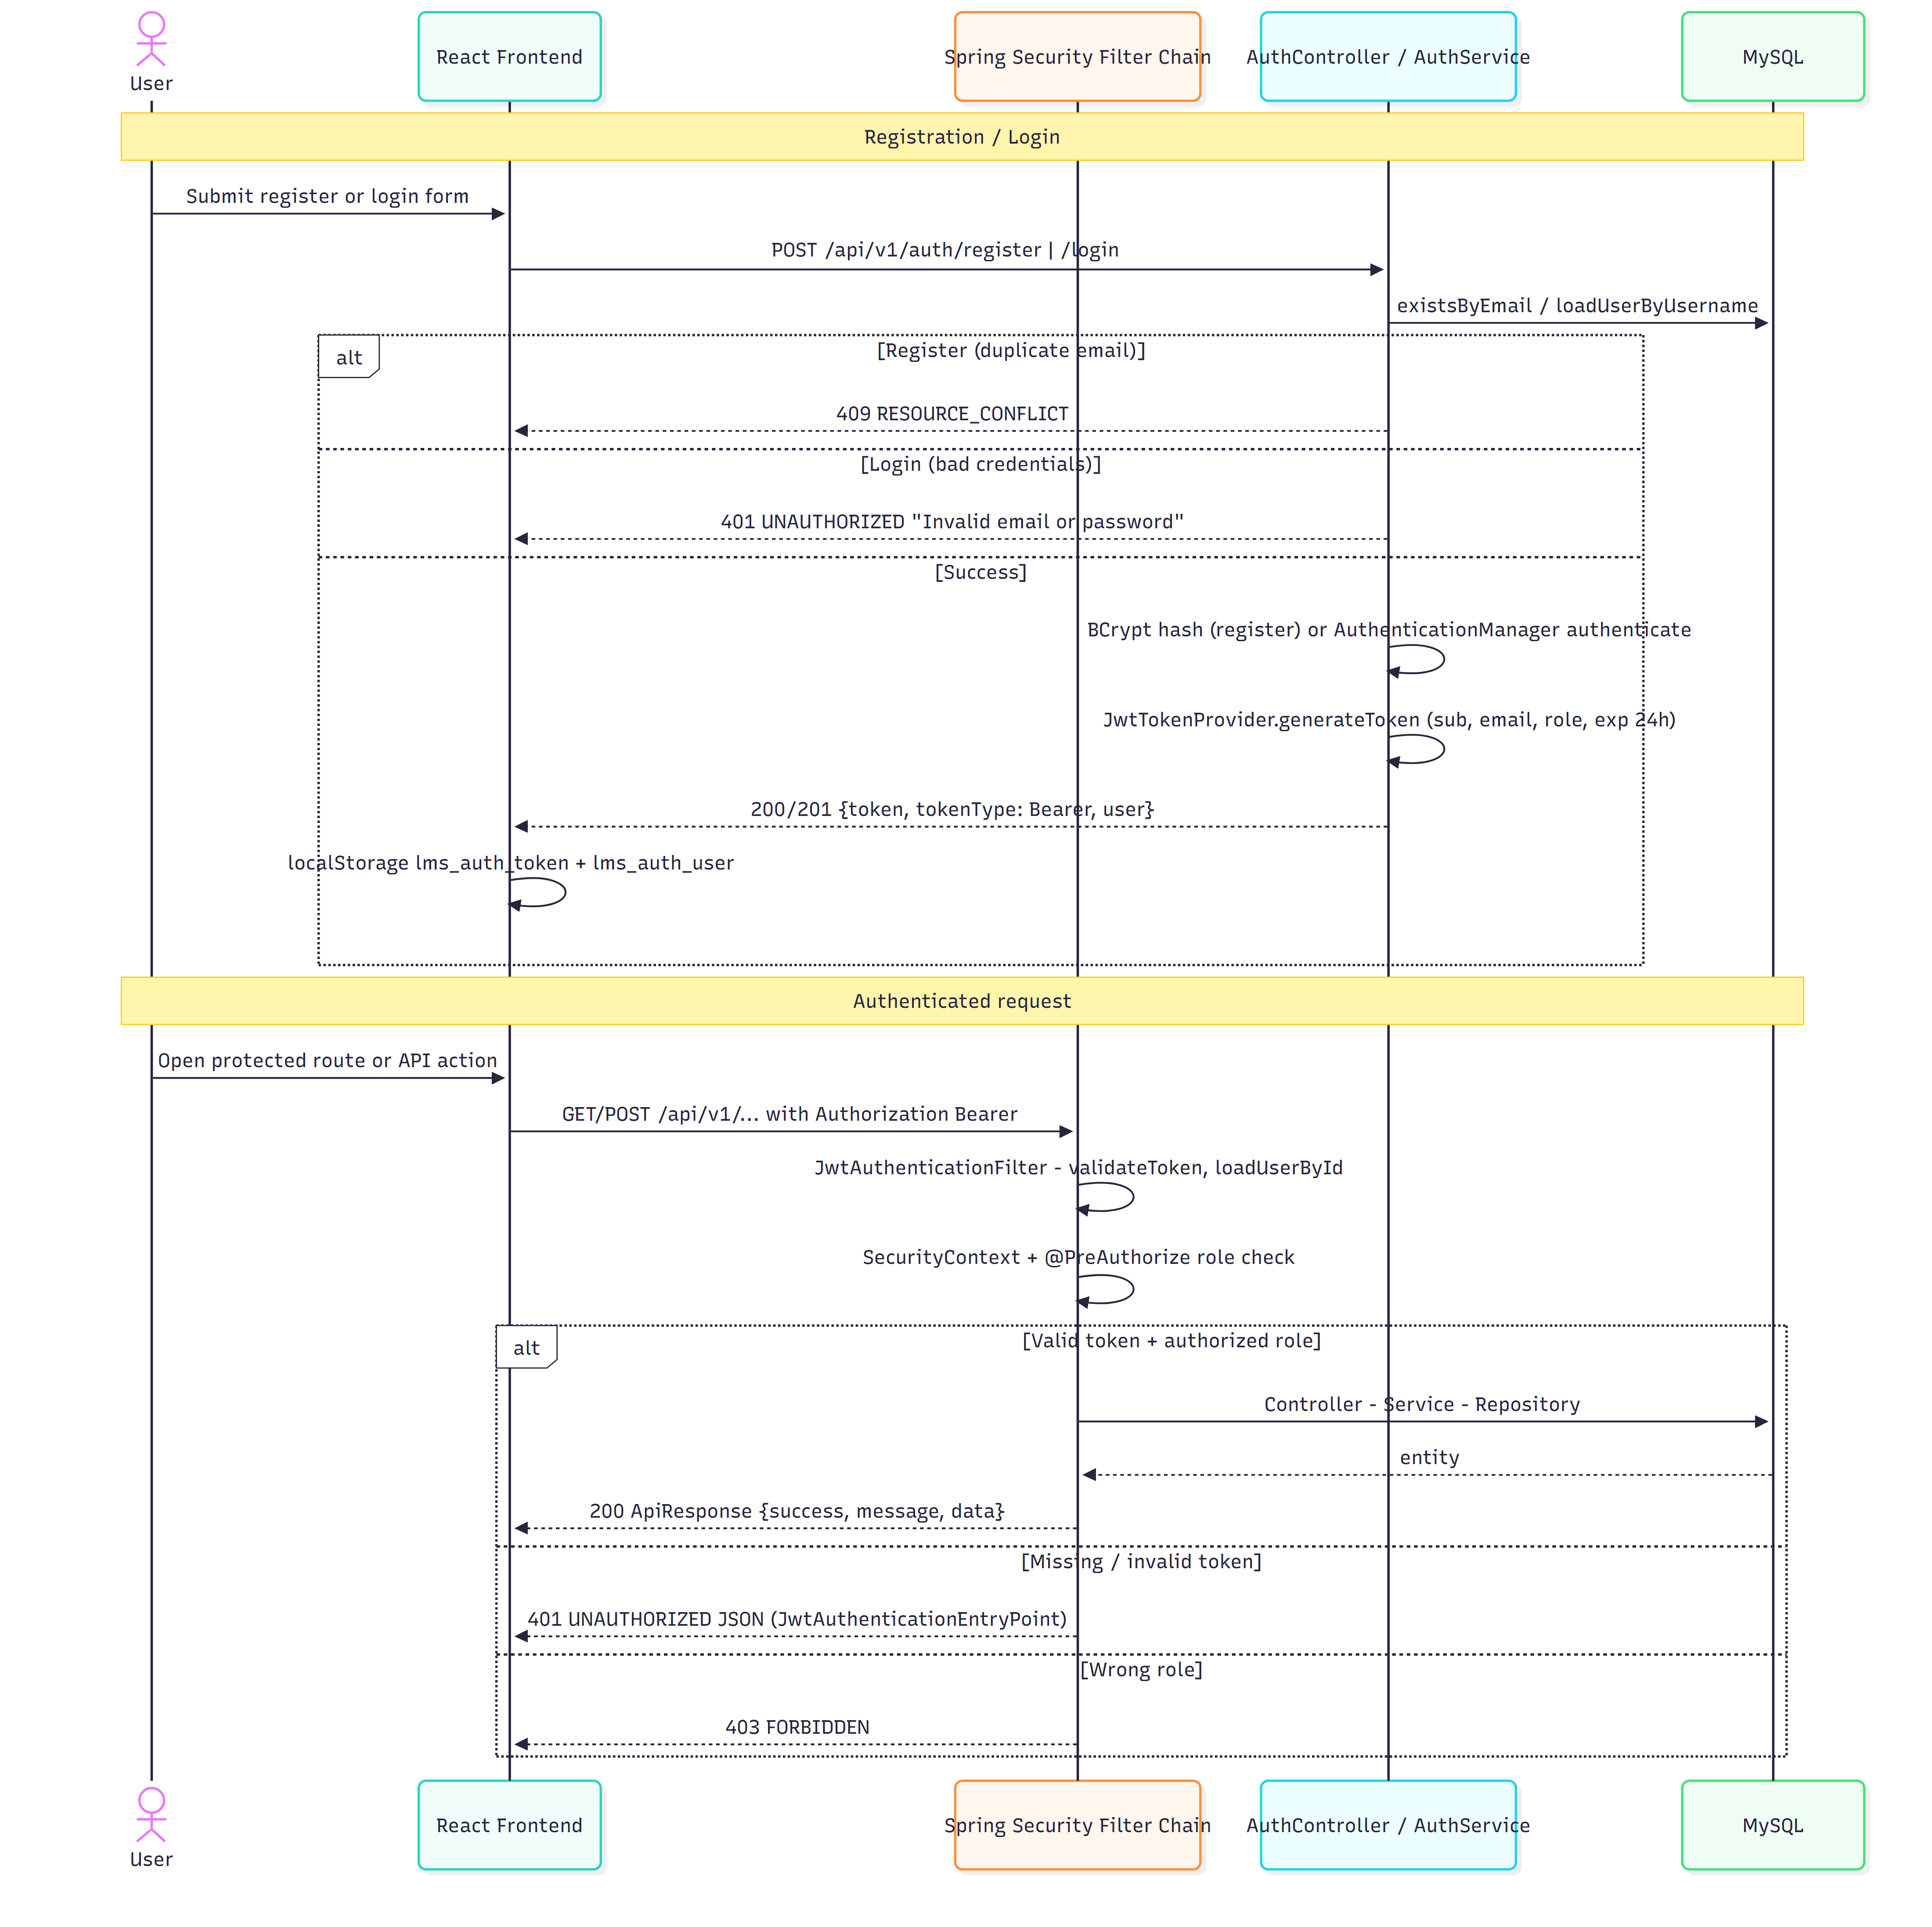
\includegraphics[width=0.95\textwidth]{diagrams/authentication-flow.png}
    \caption{Authentication and authorisation control flow}
    \label{fig:auth-flow}
\end{figure}

\begin{figure}[H]
    \centering
    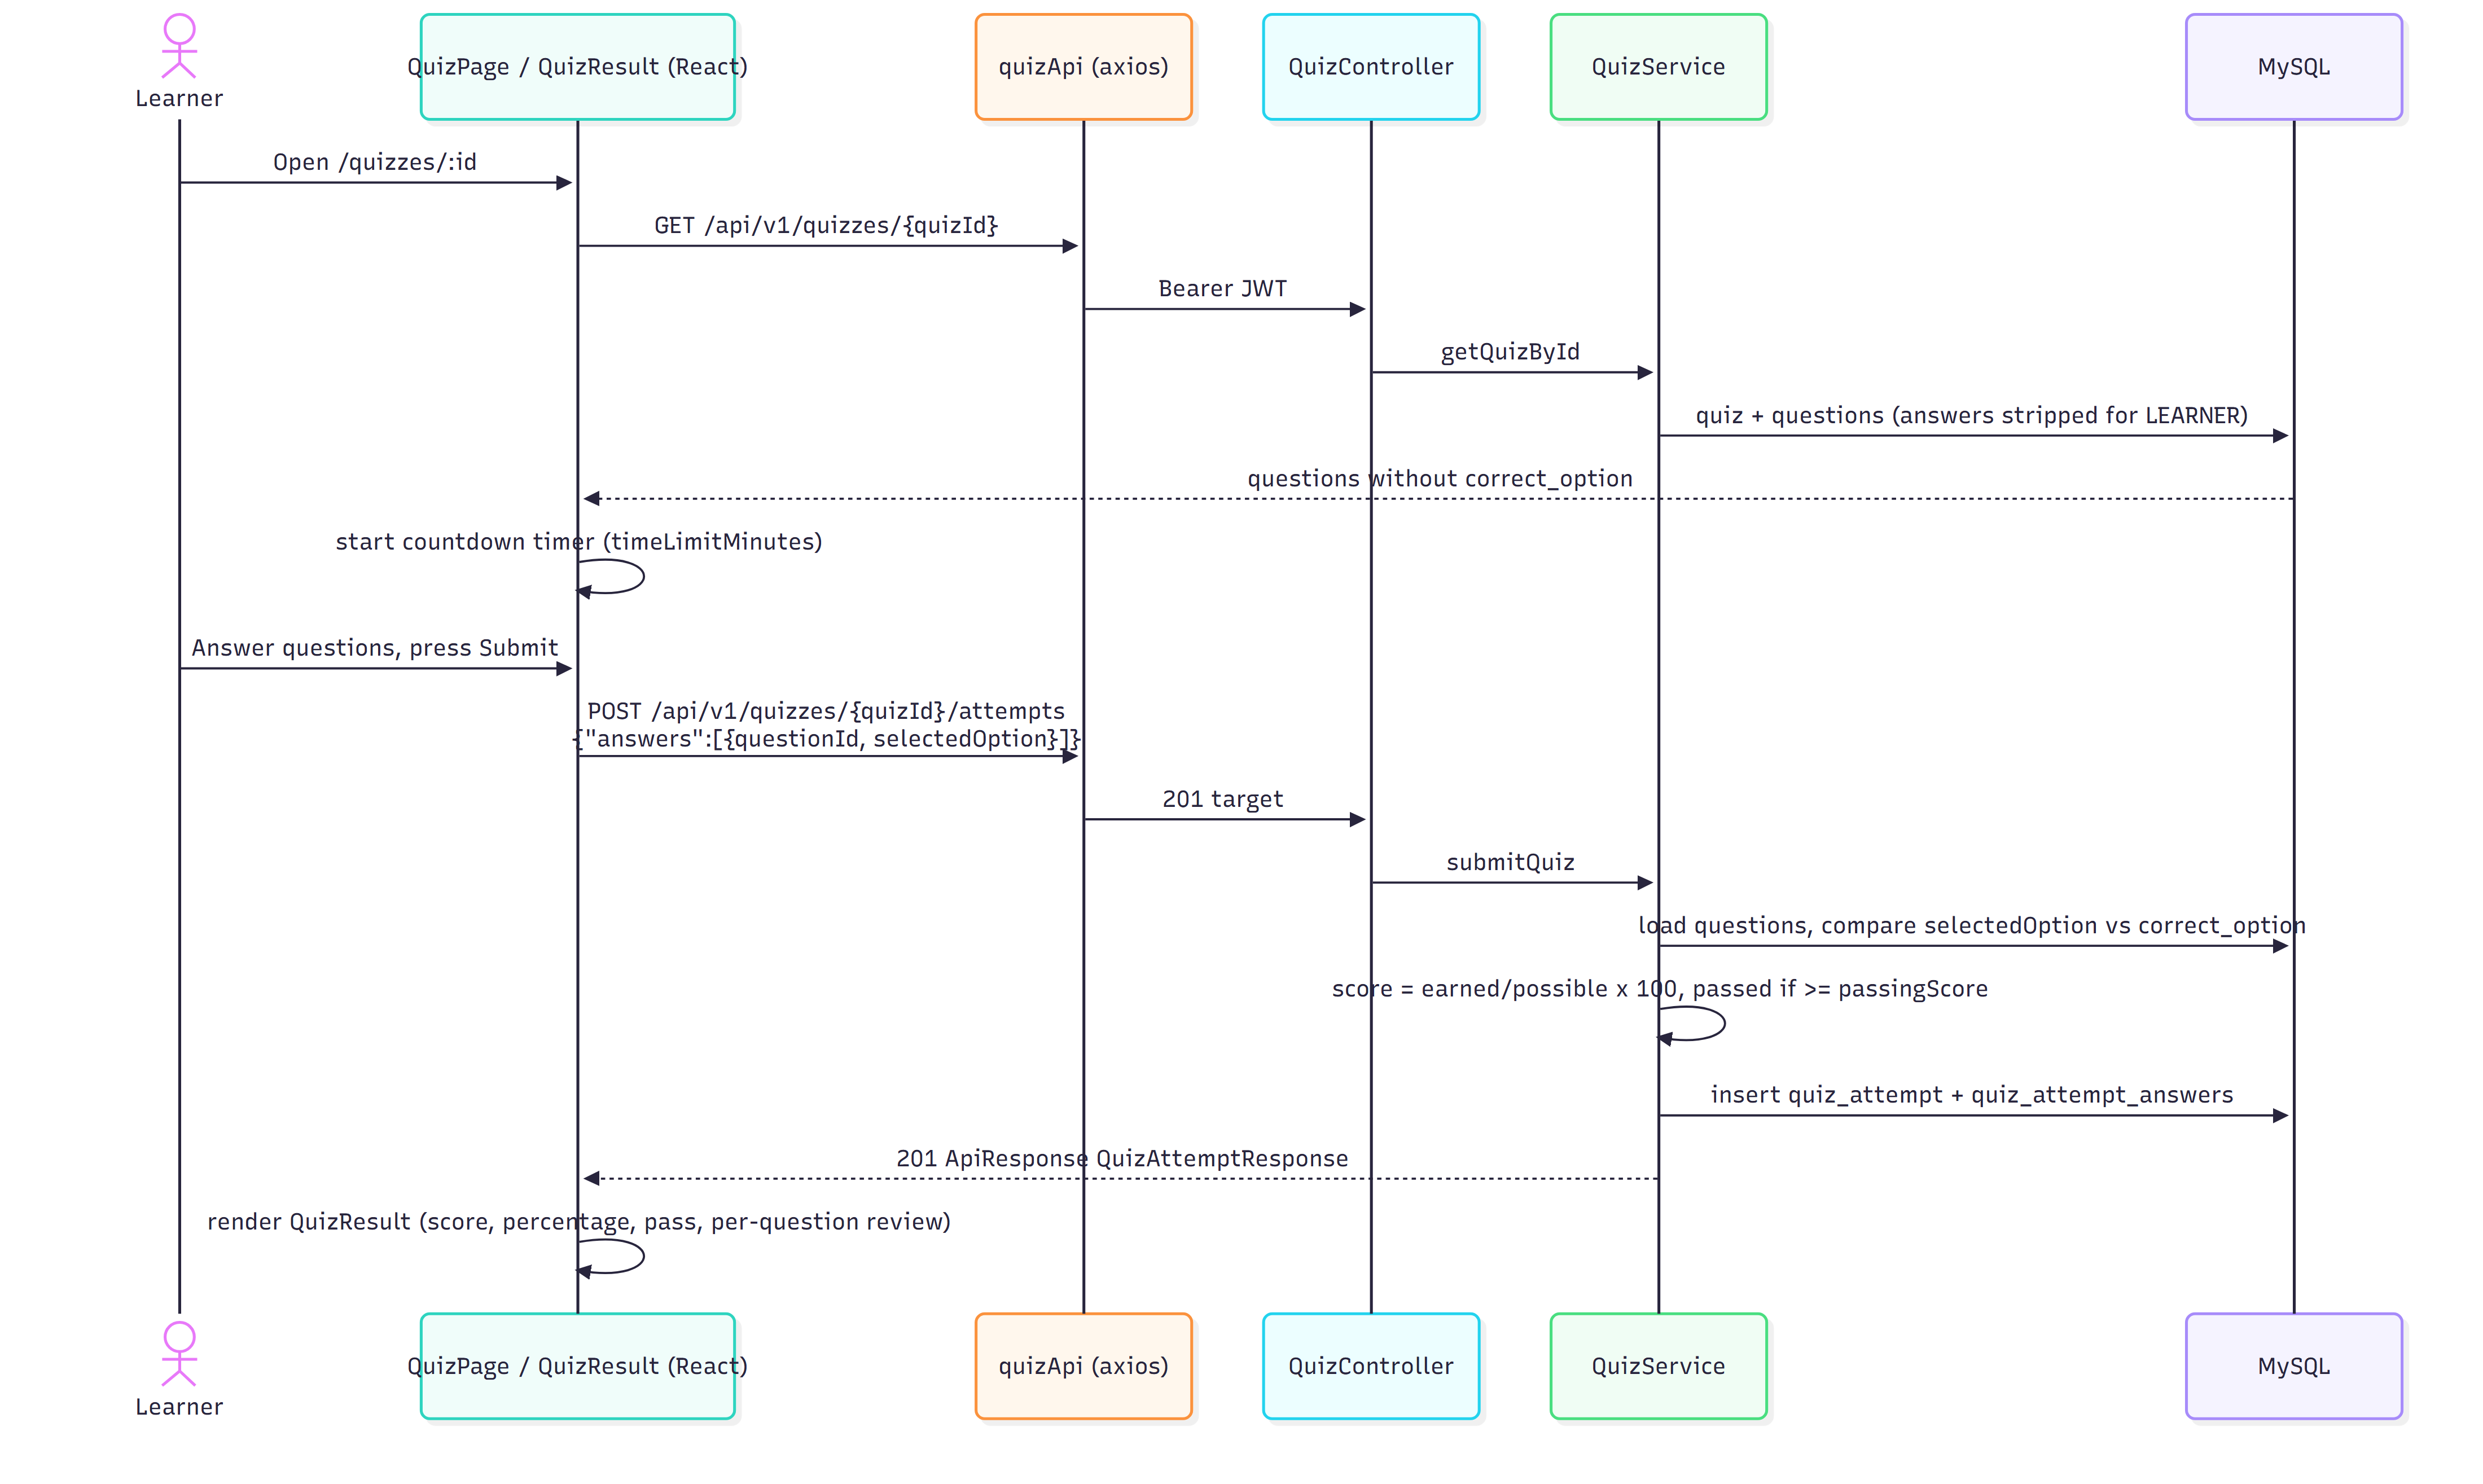
\includegraphics[width=0.95\textwidth]{diagrams/quiz-submission-sequence.png}
    \caption{Quiz submission sequence -- server-side authoritative scoring}
    \label{fig:quiz-sequence}
\end{figure}

\subsection{API surface overview}
\status{IMPLEMENTED}

47 mapped endpoints across 11 controllers (detail in Section~\ref{sec:api-documentation}):

\begin{table}[H]
\centering
\caption{API surface by domain}
\label{tab:api-surface}
\begin{tabular}{@{}L{4.6cm}C{2.0cm}C{2.4cm}L{4.2cm}@{}}
\toprule
\textbf{Domain} & \textbf{Endpoints} & \textbf{Base path} & \textbf{Public access?} \\
\midrule
Authentication & 3 & \code{/api/v1/auth} & Yes (register, login, logout) \\
Users & 3 & \code{/api/v1/users} & No (list is ADMIN-only) \\
Courses & 5 & \code{/api/v1/courses} & GET only \\
Categories & 5 & \code{/api/v1/categories} & GET only; writes ADMIN-only \\
Lessons & 5 & \code{/api/v1} & No \\
Enrollment & 3 & \code{/api/v1} & No \\
Progress & 3 & \code{/api/v1} & No \\
Quizzes \& attempts & 7 & \code{/api/v1} & No \\
Discussions & 4 & \code{/api/v1} & No \\
Feedback & 3 & \code{/api/v1} & No \\
Certificates & 2 & \code{/api/v1} & No \\
\bottomrule
\end{tabular}
\end{table}

\subsection{Data contracts}
\status{IMPLEMENTED}

\begin{lstlisting}[language=json,caption={Standard success and error envelopes (ApiResponse.java, ErrorResponse.java)}]
{"success": true, "message": "Login successful",
 "data": {"token": "eyJhbGciOi...", "tokenType": "Bearer",
          "user": {"id": 1, "email": "learner@example.com", "role": "LEARNER"}}}

{"error": {"code": "VALIDATION_ERROR",
           "message": "Validation failed for one or more fields",
           "details": ["email: must be a well-formed email address"]}}
\end{lstlisting}

\subsection{State management design}
\status{IMPLEMENTED}

\begin{itemize}
    \item \textbf{Server state} lives in MySQL; the client refetches after mutations (no global client cache such as React Query).
    \item \textbf{Session state} is two \code{localStorage} keys (\code{lms_auth_token}, \code{lms_auth_user}) mirrored into React context on mount.
    \item \textbf{URL state} encodes classroom and workspace context (\code{?lesson=}, \code{?problem=}, \code{?redirect=}).
    \item \textbf{Component state} (loading/error/data) is local to pages; no Redux/Zustand store exists.
\end{itemize}

\subsection{Error handling design}
\status{IMPLEMENTED}

\begin{enumerate}
    \item Backend: controller/service throws typed exceptions $\rightarrow$ \code{GlobalExceptionHandler} maps to status + code + message (+ field details for validation).
    \item Transport: Axios response interceptor normalises errors into \code{enhancedError} with \code{code}, \code{status}, \code{details}; network failures map to \code{NETWORK_ERROR}; timeouts use the 15\,000 ms limit.
    \item UI: \code{ErrorState} renders title/message/retry; per-action failures surface as antd \code{message.error} toasts.
\end{enumerate}

\noindent \textbf{Known gap:} HTTP 401 responses do not clear the stored session or redirect to login (\pathref{frontend/src/api/client.js}) -- logged out users with stale tokens see repeated failures until they log out manually. \status{IMPLEMENTED (defect)}
